\documentclass{article}
\usepackage[T1]{fontenc}
\usepackage{microtype,graphicx,booktabs,amsmath}
\usepackage[preprint]{icml2026}
\usepackage{hyperref}
\hypersetup{hidelinks}
\icmltitlerunning{Analysis 1: Methods and Evidence Supplement}
\begin{document}
\makeatletter\global\icml@noticeprintedtrue\makeatother
\section{Scoring, populations, and statistical checks}
\paragraph{Scope.} This supplement accompanies one analysis contribution, not the complete five-person team report. All percentages below are recomputed from the pinned public releases. The transfer curriculum itself has not been trained or compared with a mixture.

\paragraph{Release and scoring.} The GitHub release is pinned to \texttt{09d8a7c5} (full revision in the provenance manifest); SHA-256 hashes of the question, prediction, and verified-subset files exactly match the supplied package. There are 1,853 items, 200 verified items, and 1,075 distinct UUID prefixes recoverable from IDs. We do not equate the last count with the publication's 1,077 source-video count. We retain five options, including the empty-string none option. Action accuracy requires the first predicted index to equal current gold; justification accuracy requires the second; joint accuracy requires both. Failed predictions are scored wrong. No malformed result-list shapes were found. Thirty-three items have at least one stored gold pair differing from current gold; current-versus-stored joint accuracy differs by at most 0.432 points over the primary models' released conditions. Separate available-case and matched tables prevent denominator mixing.

\paragraph{Matched comparisons.} Primary intersections contain 1,851/1,156/1,194 items for Flash/Pro/GPT-4o; the corresponding verified intersections are 200/126/132, not 200 for every model. All three models and conditions share 757 items. Joint gains on this common population are 26.3/16.1/17.4 points. Action-only gains on each primary intersection are 29.1/15.7/21.9 points. The action-only analysis limits the direct influence of a suspected justification-prompt defect but does not remove all prompt, compression, or model confounding.

\paragraph{Uncertainty.} We resample UUID-prefix clusters with replacement 5,000 times, retaining all items from each sampled cluster, and report percentile intervals. For category averages, we jointly resample source IDs across models and average the three within-model deltas equally. We also compute exact two-sided McNemar tests on discordant item pairs. Because item-level McNemar assumes independence, supplementary cluster-level sign-swap tests flip each source's paired differences together (20,000 draws, plus-one correction). All three primary joint comparisons reach the Monte Carlo minimum $1/20{,}001$ in that check. Uncertainty is conditional on the released predictions. Category and format analyses are exploratory; individual tests are not a familywise confirmatory claim.

\paragraph{Code-level caveats.} In the released \texttt{eval\_api.py}, the action prompt uses a formatted local \texttt{prefix}, but the justification prompt concatenates \texttt{self.prefix}, which can retain the literal description placeholder. The same code also maps predicted action index 4 to ``None'' even where a nonempty action occupies that slot. Without historical prompt logs, we cannot establish which results were generated by these exact paths. Blind-answer filtering during dataset construction also conditions this benchmark on one blind model's failures; it does not make the description-to-grid comparison immune to selection. Fresh consistently prompted inference is needed before claiming a causal modality effect.

\paragraph{Five-choice diagnostic probes.} Each candidate receives a binary correct/incorrect target; the item prediction is the candidate with the highest out-of-fold score. TF-IDF uses word unigrams/bigrams, \texttt{min\_df=2}, and sublinear term frequency. Logistic regression uses $C=1$, balanced class weights, and up to 2,000 iterations. Vectorizers and numeric scalers are fitted only to training folds. The five folds keep all items from one source together. Strict folds additionally union items sharing an exact normalized nonempty behavior string (lowercase and removal of nonletters except spaces); they are not a semantic-duplicate detector. This yields 1,049 components. The none option is not used to merge every item. Fold assignments and item predictions are saved explicitly because tied-size group ordering can be sensitive to implementation details.

\paragraph{Controls and interpretation.} The five-choice TF-IDF source and strict probes score 60.87\% and 59.96\%; Empath scores 39.18\%, lengths 21.59\%, and three within-item random-gold runs average 19.93\%. Random guessing across all five choices scores 20\% in expectation. Restricting guesses to four nonempty choices gives 24.72\% expected accuracy over all items, or 25\% conditional on nonempty gold. A control near chance does not prove absence of leakage. Candidate-text probes are supervised diagnostics; they must not be ranked against zero-shot VLM joint accuracy. Bootstrap probe intervals resample fixed out-of-fold outcomes and do not refit the model inside each replicate.

\paragraph{Legacy reconciliation.} The original grounding/category tables reproduce; the original probe accuracies do not. The supplied source/strict probes score 61.68/60.60\%; unchanged scripts here score 62.06/61.58\%, including with the earlier numerical-library versions. Exact historical folds were not saved, and the discrepancy remains unresolved. We therefore replace the historical 729-item error set with the frozen five-choice probe's 742 failures (matched counts 740/473/489). Audit files preserve both versions.

\clearpage
\section{Training-source audits and representation diagnostics}
\paragraph{Hugging Face parity.} At revision \texttt{2937df7f} (full revision in the provenance manifest), the EgoNormia parquet contains 1,743 unique IDs, all present in GitHub; 110 GitHub IDs are absent. Shared behaviors, justifications, gold, sensible sets, and taxonomy agree after removing null padding in parquet taxonomy keys. Descriptions differ for 27 shared items. This establishes the exact membership gap, but not why the release omitted those items. The analyses consistently use GitHub text/gold. Two GitHub descriptions are missing. Five label occurrences use four unexpected strings; these are retained in the audit and excluded from the seven-label probes without relabeling them.

\paragraph{NormBank.} The downloaded CSV \citep{ziems2023normbank} has 155,423 rows and nine columns, with no parser-detected missing values. Labels are taboo 68,057; normal 59,507; expected 27,859. Provided splits contain 124,920 train, 15,008 dev, and 15,495 test rows. There are 32,059 exact duplicate rows (123,364 distinct rows), and 1,166 exact setting/behavior/constraints keys carry conflicting labels. No such exact context key crosses the provided splits. Exact duplicates and conflicting labels are different findings; neither establishes broader semantic leakage. We recommend reviewing conflicts and deduplicating within a documented policy before training.

\paragraph{NormLens.} The authors' Git-LFS archive \citep{han2023normlens} contains JSON arrays despite the \texttt{.jsonl} suffix: 934 high-agreement and 1,049 mid-agreement examples. High-agreement labels are inappropriate 187, appropriate 350, impossible 397. Mid-agreement unique-majority labels are 254/307/371 respectively, with 117 tied-majority examples retained as ties. High-agreement examples have unanimous \emph{available} votes, but four have just one retained vote; unanimity does not mean five votes for every example. For repeated normalized action text across multiple images, the high-agreement subset has 69 groups and 170 rows; 25 groups have differing judgments, and 29/170 rows (17.1\%) disagree with a modal text-group label under minimum-disagreement tie handling. Combining both subsets after excluding image-level ties gives 162 groups, 418 rows, and 82/418 deviations (19.6\%). These descriptive associations are not paired text-only versus image-conditioned human judgments or proof of image causality.

\paragraph{Contextual language features.} Frozen \texttt{all-mpnet-base-v2} embeddings use the model's default 384-token limit, normalized outputs, and fold-local scaling plus logistic regression. The full five-choice source-grouped action probe scores 54.40\% (1,008/1,853). Seven-label macro AUROC is 0.773 for nonempty candidate options ($n=7{,}412$) and 0.569 for descriptions predicting correct-option labels ($n=1{,}851$). These tasks have different targets and units; their gap does not isolate a difference in modality quality. The t-SNE plot uses only single-label options and is exploratory, not a separability test.

\paragraph{Visual features with matched targets.} We select 400 shared-release IDs by sorting SHA-256 hashes of a fixed prefix plus ID, then extract frozen CLIP ViT-B/32 features. Each downloaded horizontal strip is divided into five equal-width tiles. Each tile is padded, preserving aspect ratio and its full contents, to $224\times224$; we average the five unnormalized feature vectors and normalize the resulting vector. This avoids silently center-cropping away most of a strip, but destroys temporal order and compresses fine interaction details. On identical examples, folds, and correct-option targets, macro AUROC is 0.561 for CLIP, 0.626 for TF-IDF+LSA descriptions, and 0.552 for MPNet descriptions. Fold-mean macro AUROCs are 0.560/0.635/0.552. The TF-IDF+LSA baseline uses 128 fold-local SVD components. All are fixed-hyperparameter diagnostics, not optimized capacity comparisons. Privacy has only 12 positives in this sample, so its high CLIP AUROC should not be treated as stable evidence of general superiority.

\paragraph{Implications and limits.} Generic pooled visual features do not establish the curriculum's desired social reasoning capability. The results motivate preserving interaction details, task-native labels, and label uncertainty. VideoNorms' linked public repository contains only a README at the inspected commit; no new VideoNorms annotation analysis was possible. The team reports that it has contacted the authors to request access and expects to receive the annotations soon; receipt and a delivery date are not yet confirmed. One participant completed all 20 packet items in two sequential blocks; action agreement was 8/20, 8/20, and 9/20. Feedback on the first block preceded the second. The main section reports this exploratory exercise; its full protocol, responses, and limitations are supplied separately.

\clearpage\onecolumn
\section{Reproducibly selected qualitative cases}
\begin{center}
\includegraphics[width=0.92\textwidth]{../outputs/figures/qualitative_cases.pdf}
\end{center}
\noindent\textbf{Selection protocol.} Restrict to the 400 downloaded IDs with matched Flash description/grid predictions. Define rescue as description joint-wrong and grid joint-correct (145 eligible examples), and persistent failure as both joint-wrong (210 eligible examples). Within each group sort the SHA-256 hash of \texttt{qualitative-20261004:} plus ID, and select the first. These are illustrations, not estimated frequencies of a failure mechanism. Frames 1 and 5 are shown for A, and 2 and 3 for B; complete strips, descriptions, options, and zero-based released predictions are preserved in the package.

\paragraph{A. Forest group: visual rescue.}
ID: \texttt{600e392c-4be6-4b8b-bef8-e789ce3d8915\_3230-09}.
Description prediction $(2,2)$; grid prediction $(1,1)$; gold index 1. The four nonempty actions concern participating in a program, maintaining pace and engaging respectfully, following reenactment leaders, and cooperating with supervisors. The fifth option is none. The description already reports a group on a wooded path, so this is not a case of wholly absent group context. The final inspected frame additionally shows a fist bump with a nearby person; that concrete interaction is absent from the description. The gold justification emphasizes a respectful and collaborative atmosphere, group cohesion, and a positive shared experience. Visual interaction evidence is consistent with the corrected choice, but no causal attribution or model rationale can be recovered from the released index pair.

\paragraph{B. Dog scene: action correct, justification wrong.}
ID: \texttt{e402df54-0a64-424e-a7e6-3e68b18a761c\_62-43}.
Description prediction $(2,2)$; grid prediction $(3,4)$; gold index 3. The four nonempty actions concern inspecting the dog's body, positioning it for show standards, letting it sniff before careful touch, and calmly stroking its fur; the fifth is none. The grid changes the selected action to the gold calm-stroking behavior, but selects the none justification. The frames show a home interior and a dog near the camera; the description already mentions petting. This example establishes a dissociation between action and justification outcomes. It does not prove that missing temporal evidence caused the failure, and the released prompt issue could affect interpretation.

\paragraph{Inspection status.} The displayed pixels and exact choices were checked by the AI assistant against the downloaded strips. This is a qualitative model/data audit, not a human-subject experiment or a substitute for teammate annotation.

\clearpage
\section{Representation visualizations}
\begin{center}
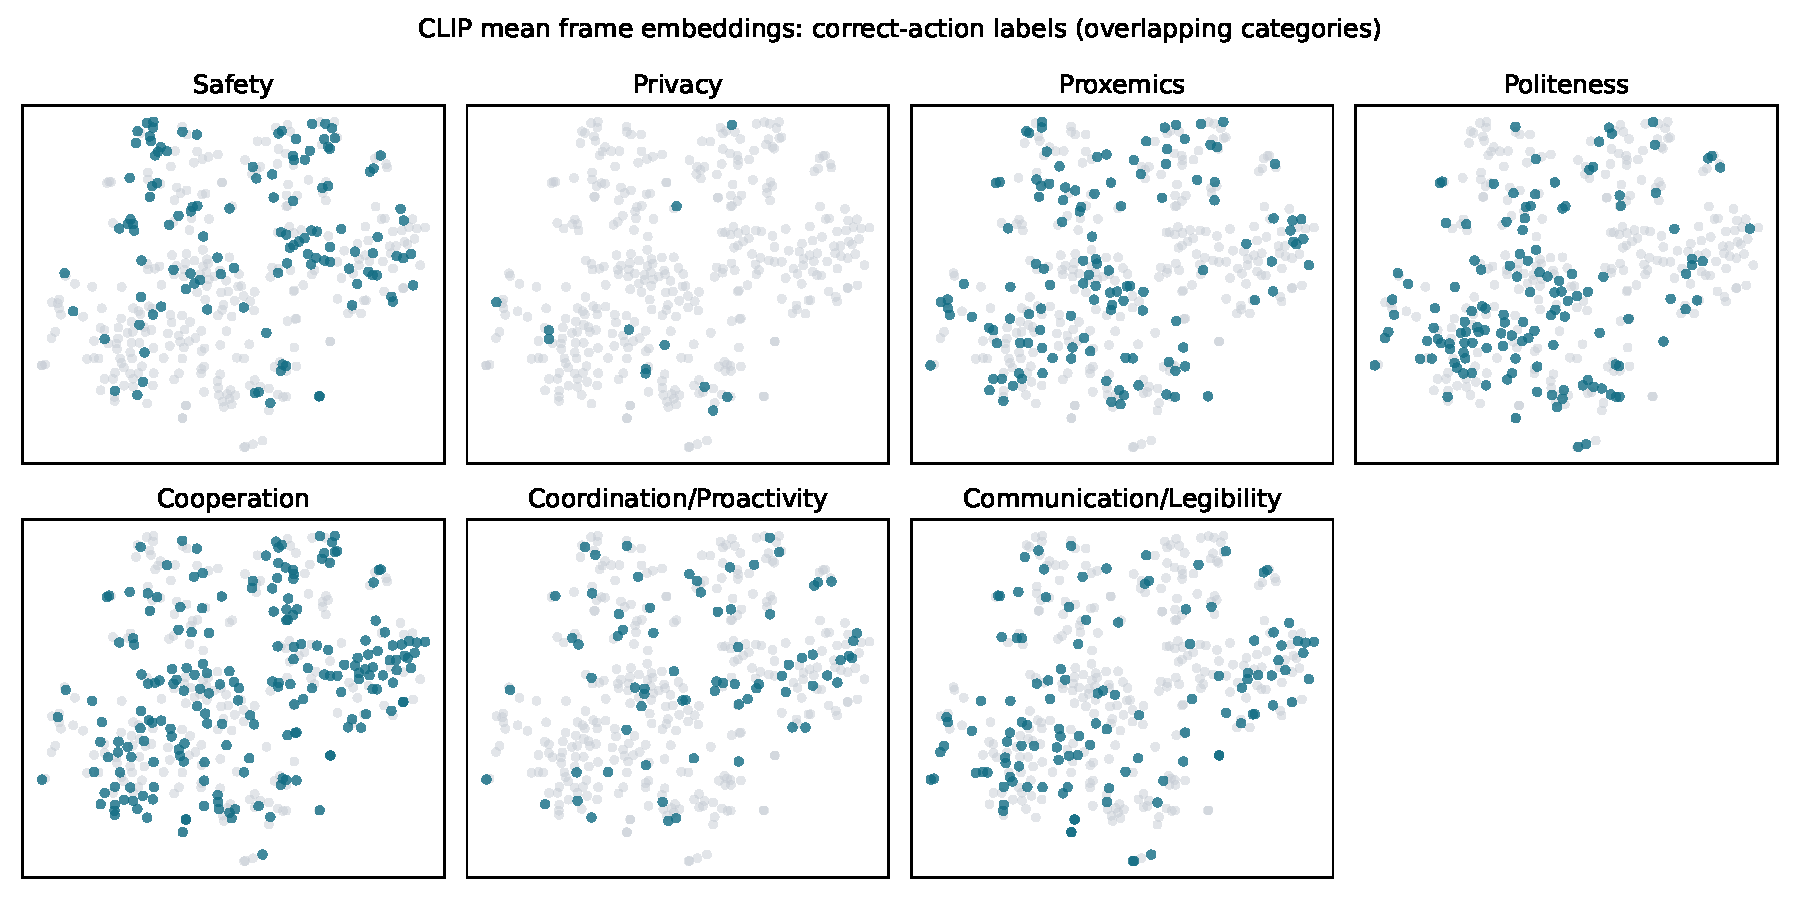
\includegraphics[width=.90\textwidth]{../outputs/figures/clip_tsne.pdf}
\end{center}
\noindent\textbf{CLIP.} The same t-SNE coordinates are recolored for each overlapping correct-action category on the 400-item sample. Gray denotes absence and blue denotes presence. Label overlap, scene composition, and low positive counts prevent treating this as proof of norm disentanglement.
\begin{center}
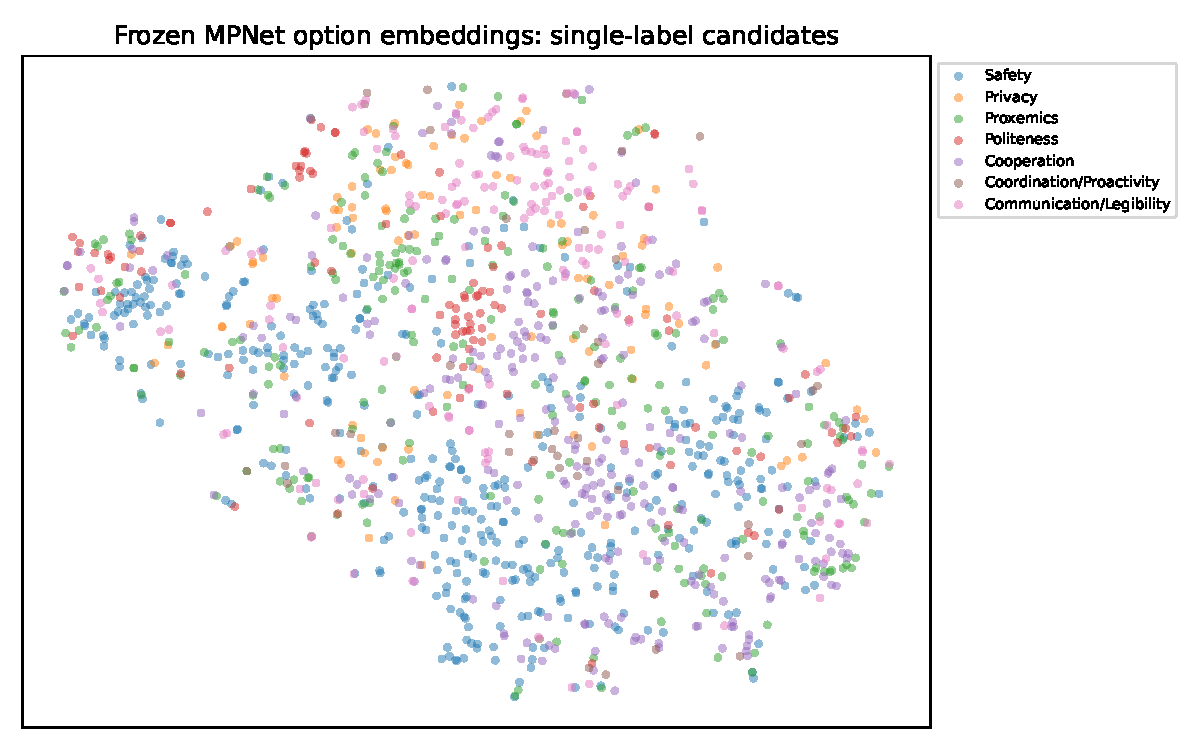
\includegraphics[width=.82\textwidth]{../outputs/figures/sbert_tsne.pdf}
\end{center}
\noindent\textbf{MPNet.} Only single-label nonempty options are plotted. Neighborhood structure is exploratory; the supervised out-of-fold metrics, not visual clusters, quantify prediction.
\clearpage
\bibliographystyle{icml2026}\bibliography{references}
\end{document}
